\chapter{Setting up the problem}

\section{The Data}

The aim of this thesis is to use deep learning techniques to segment CT scans of the chest and identify the voxels that are in the part of the heart called the atrium. The atrium is composed of two chambers called the right and left atrium which are the two entry points of the blood into the heart, one returning to the heart to complete the circulating cycle through the body and the other coming back from the lungs after being oxygenated.\\

The data from which the training and testing datasets are generated comprise 27 chest computerised tomography (CT) scans. CT scans are 3 dimensional grey scale images generated via computers combining many X-ray images taken from different angles to produce cross-sectional images of specific body parts. They are stored as DICOM files, DICOM standing for Digital Imaging and Communications in Medicine and which is a standard for handling, storing, printing, and transmitting information in medical imaging. Each has been segmented by trained radiologists at St Thomas's hospital, the results of which are stored in Nearly Raw Raster Data (NRRD) files, a standard format for storing raster data. These are 3D arrays of the same dimension, each voxel taking either or two values which indicates whether the corresponding voxel in the CT scan is in the Atrium (1) or not (0). 

\section{Generating the datasets: The Tri-Planar Method}

Classifying the voxels require building an input set for each containing enough local and global information to allow the Neural Network to learn effectively. One way of providing 3 dimensional information is to use the so-called tri-planar method [reference the paper that started it on knee cartilage]. This consists in generating 3 perpendicular square patches of a given dimension in the transversal, saggital and coronal planes centred at the voxel of interest (see the figure). This standard technique has been found to give competitive results compared to using 3D patches while being much more computationally and memory efficient. In addition, we use a multiscale approach where we add 3 more input channels composed of compressed patches that are originally 5 times larger than the above set of patches resized to the same size to provide global information about the surroundings of concerned voxel.\\

Each patch is fed into a different input channel of the Convolutional Neural Network with one or more convolutional layers. The outputs of those channels are then feed as input to a number of connected layers before a classifying layer as output layer.

\begin{figure}
\centering
\begin{minipage}{0.45\textwidth}
\centering
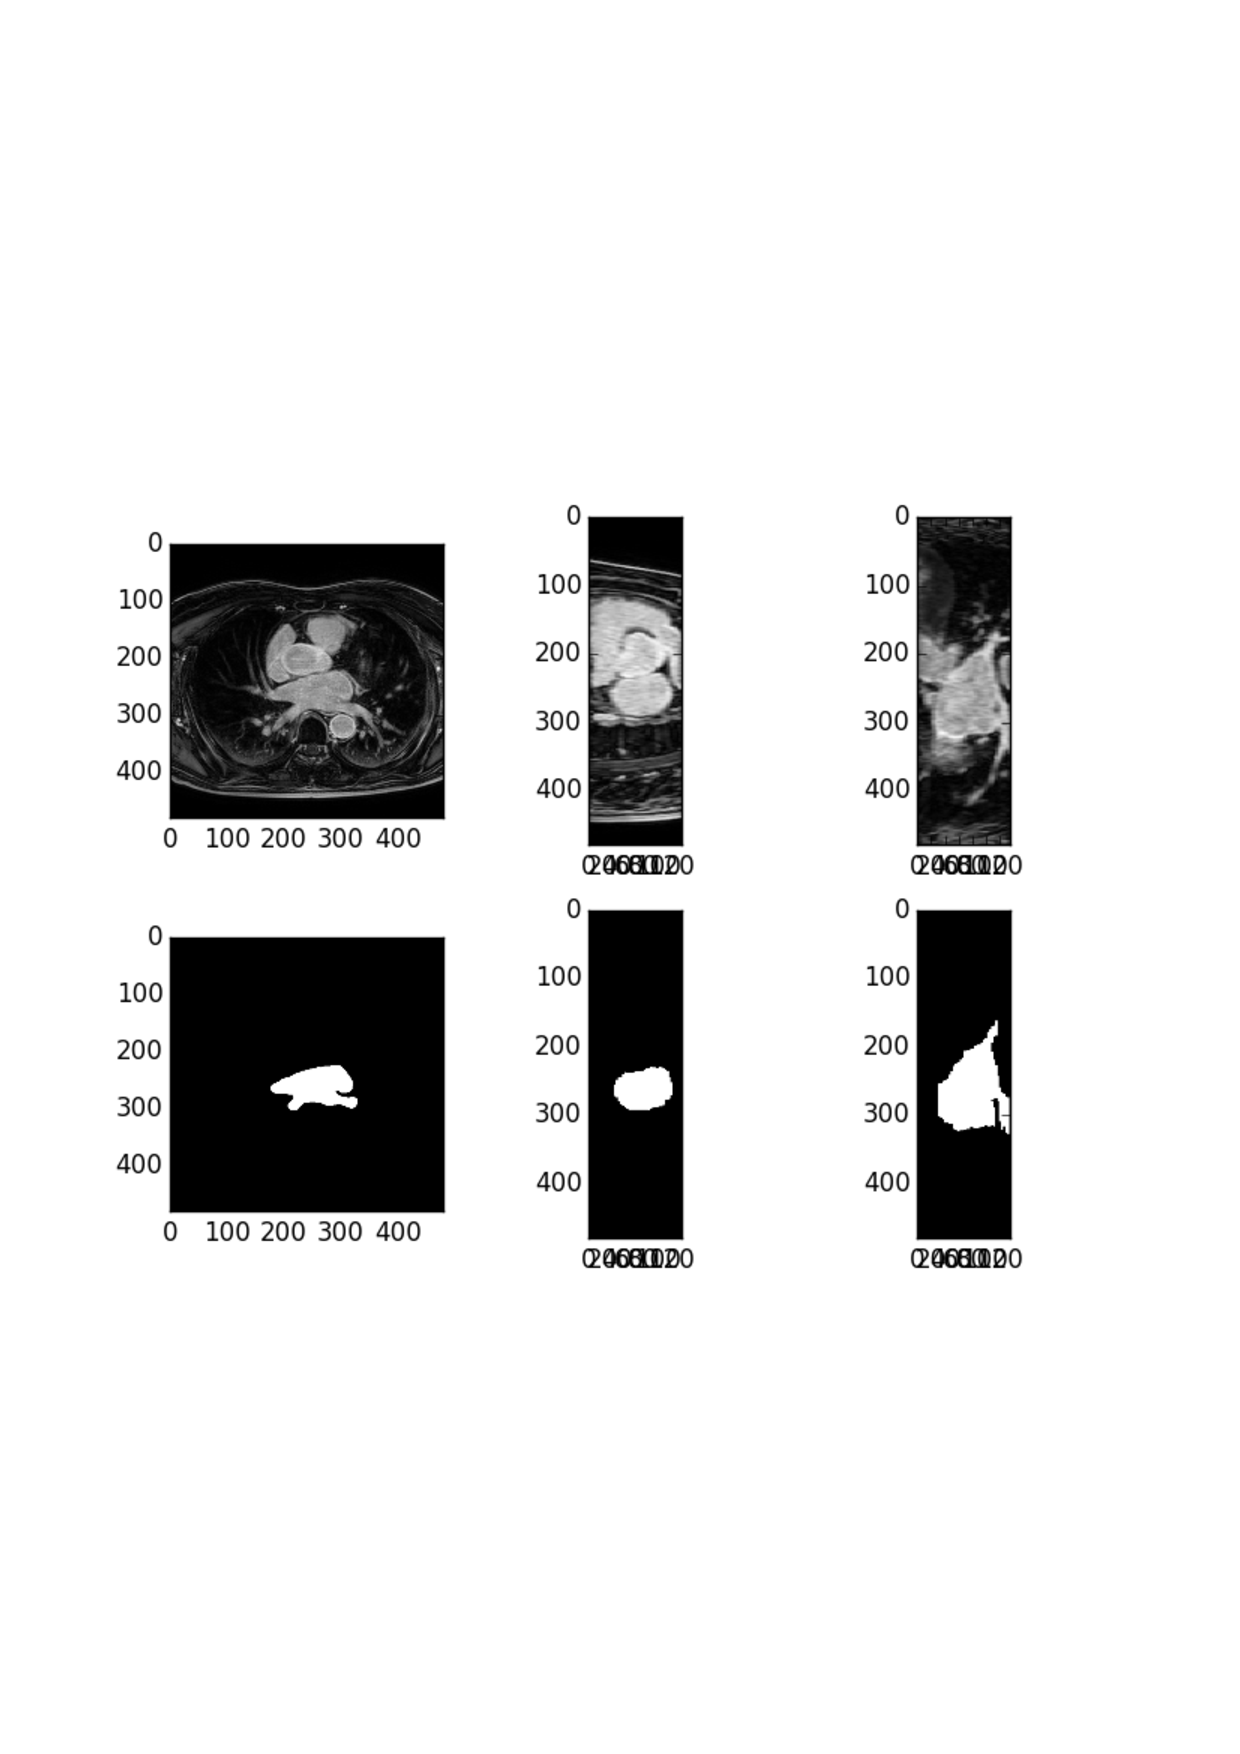
\includegraphics[trim=2cm 8cm 2cm 8cm, clip=true, height=60mm]{Chapter2/example_slice.pdf}
\end{minipage}\hfill
\begin{minipage}{0.45\textwidth}
\centering
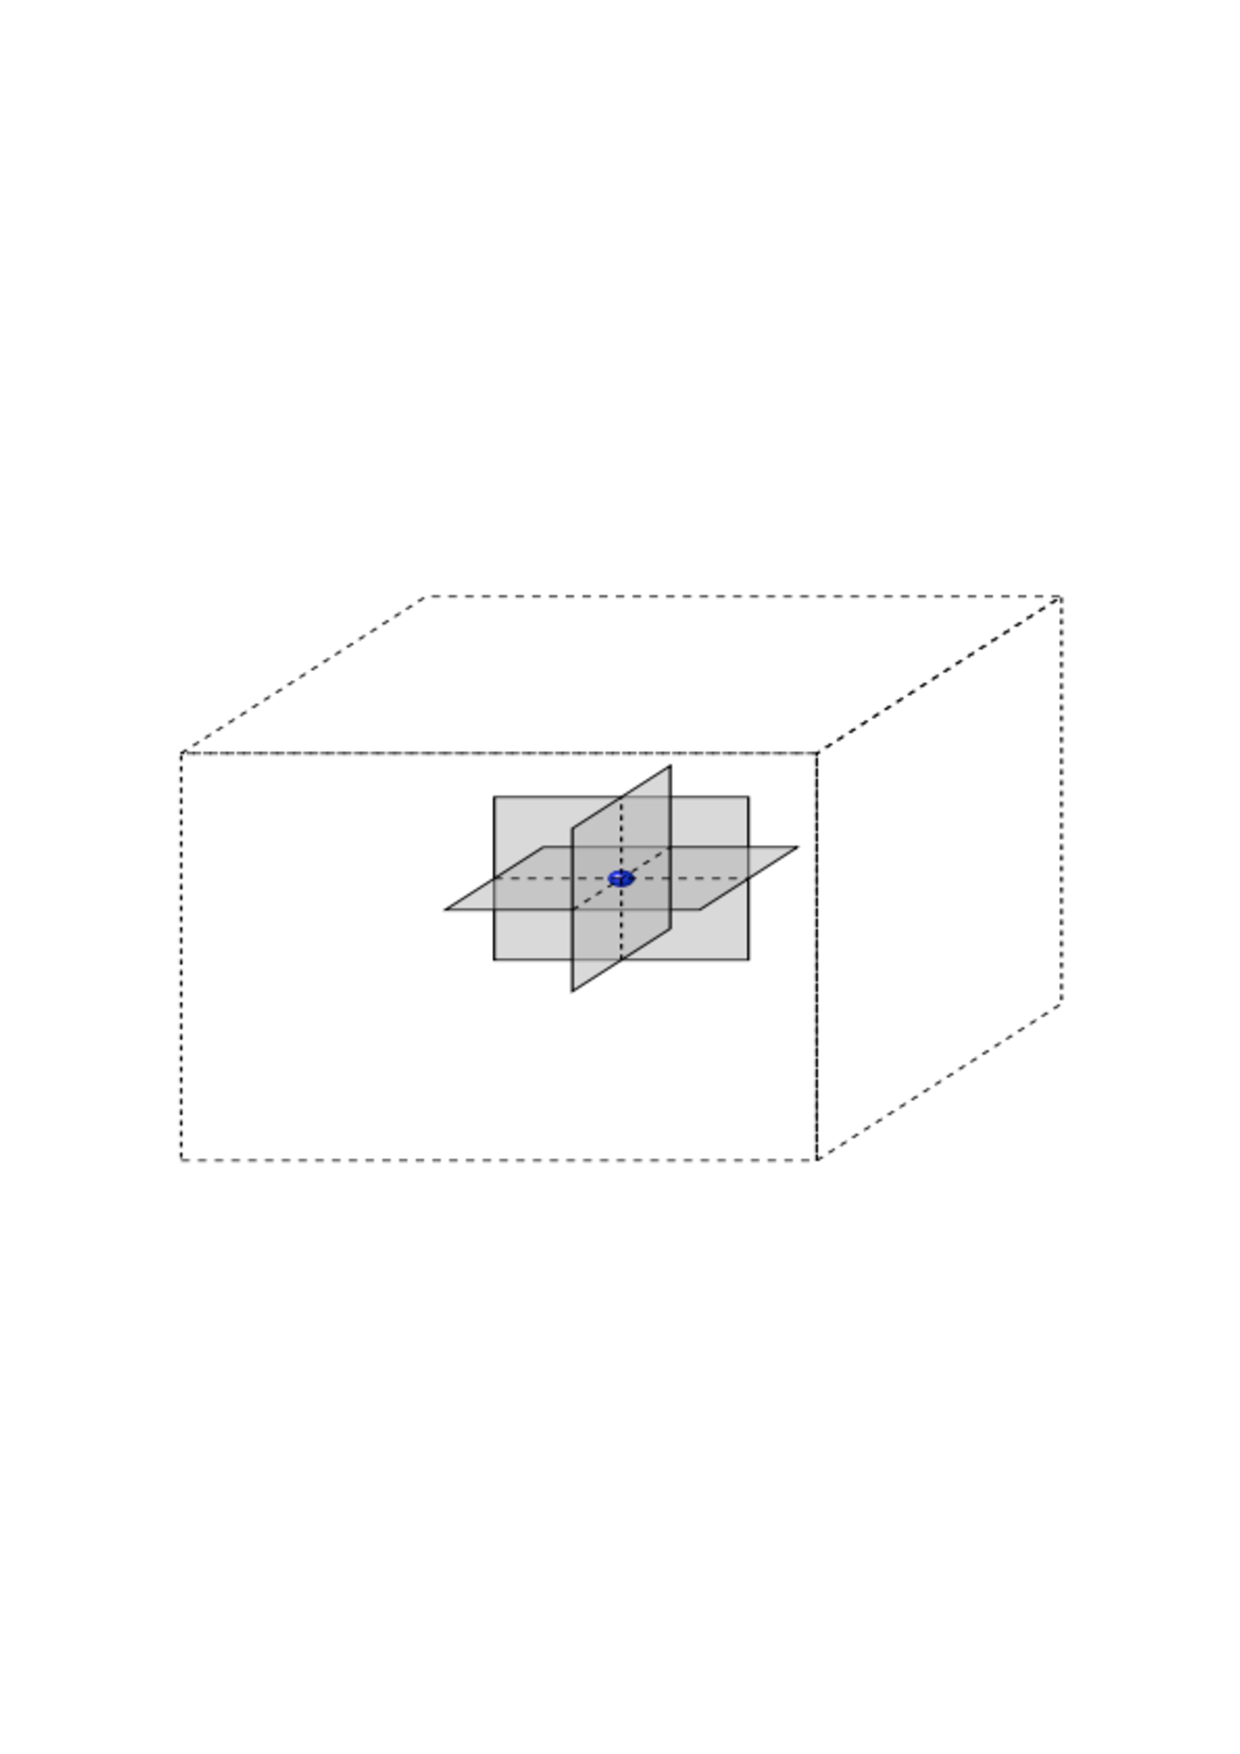
\includegraphics[trim=2cm 8cm 2cm 8cm, clip=true, height=60mm]{Chapter2/triplanar.pdf}
\end{minipage}
\caption{Left: grey scale slices from a CT scan taken in the transversal, saggital and coronal planes. Right: illustration of the triplanar}
\end{figure}

\section{Implementation Details}

\subsection{Libraries}

We use Torch, an open-source library maintained by Facebook in Lua aiming to provide a Matlab-like environment for scientific computing, along with a number of dependent libraries (cunn, cudnn, fbcunn) to train the convolutional networks on single and multi-GPUs. In addition, we use Python and a number of its libraries to handle all the logistics from generating the datasets to producing plots of segmentation results.

\subsection{Computer Power}

The training of the CNNs were conducted on 2 multi-GPU clusters, named montana-nvidia and montana-k80, kindly provided by Prof. Montana's laboratory. montana-nvidia consists 24 cores with 129 Gb of memory connected to two NVIDIA Tesla K40m and two Tesla K20Xm while montana-k80 on the other hand has 56 cores with 258 Gb of memory supported by 8 of NVIDIA's Testla K80. 














